\documentclass{article}

% Langue
\usepackage[utf8]{inputenc}
\usepackage[T1]{fontenc}      
\usepackage[francais]{babel}

% Mise en forme générale
\usepackage[top=2.5cm,bottom=2.5cm,right=2.5cm,left=2.5cm]{geometry}

% Package divers
\usepackage{chemist} 
\usepackage[version=3]{mhchem}
\usepackage{chemfig}
\usepackage[squaren, Gray]{SIunits}
\usepackage{sistyle}
\usepackage[autolanguage]{numprint}
\usepackage{url}
\usepackage{rotating}
\usepackage{xcolor,colortbl}
\definecolor{Gray}{gray}{0.85}

\usepackage{hyperref}
\hypersetup{
    colorlinks,
    citecolor=black,
    filecolor=black,
    linkcolor=black,
    urlcolor=black
}

% Nouvelles commandes
\newcommand{\std}{\ensuremath{^{\circ}}}
\newcommand\ph{\ensuremath{\mathrm{pH}}}
\newcommand{\annexe}{\part{Annexes}\appendix}
\newcommand{\biblio}[1]{\bibliographystyle{plain}\bibliography{#1}\nocite{*}}

\newcommand{\doctitle}[1]{
	\title{#1}
	\author{\textbf{Groupe 124.3}\\
	\textsc{Frenyo} Péter (6266-12-00)\\
	\textsc{Gillain} Nathan (7879-12-00)\\
	\textsc{Lamine} Guillaume (7109-13-00)\\
	\textsc{Piraux} Pauline (2520-13-00)\\
	\textsc{Paris} Antoine (3158-13-00)\\
	\textsc{Quiriny} Simon (4235-13-00)\\
	\textsc{Schrurs} Sébastien (7978-13-00)}
	\date{\today}

	\begin{document}

	\maketitle
	\tableofcontents
}

\doctitle{Tache 4 : Etude HAZOP du noeud autour du réacteur de synthèse d'ammoniac}

\section{Dangers présentés par les substances mises en oeuvre durant la synthèse de l'ammoniac}
\subsection{L'azote}
Premièrement, le diazote utilisé est gardé sous pression. Tout gaz comprimé présente un danger. 
En effet, des rejets de gaz comprimé mal contrôlés dans les réacteurs chimiques peuvent entraîner 
la rupture des cuves, créer des fuites dans l'équipement ou les canalisations ou faire emballer la réaction \cite{canada}.
Si le contenant du gaz n'est de plus pas solidement fixé, cela peut entraîner un effet dit "fusée" 
et causer des dommages et blessures.

Le diazote est également un gaz toxique et peut entraîner des morts par asphyxie dans les espaces confinés. 
%il est nécessaire de vérifier la présence d'une proportion suffisante d'oxygène dans de tels espaces confinés 
%avant d'y pénétrer, ou de s'équiper d'un appareil respiratoire autonome. (Wikipedia) < Voit si tu veux rajouter ça en plus, ou c'est plutôt une solution.

\subsection{L'hydrogène}
Les dihydrogène étant également comprimé, il présente les même dangers de gaz sous 
pression que mentionnés pour le diazote.

De plus, le dihydrogène est un gaz extrêmement inflammable, réactif et explosif. 
Un choc, une étincelle ou autre peut facilement 
entraîner une combustion rapide pouvant mener à une explosion.

L'hydrogène peut également corroder certains métaux et être source de fragilités
ou fissures sur le matériel, et présente un danger de suffocation par inhalation.

\subsection{L'argon}
L'argon étant également maintenu sous pression, les même dangers que ceux mentionnés
pour l'azote sont présents.

L'argon en forte concentration peut réduire la teneur en oxygène du milieu,
provoquant des pertes de consciences ou, dans le pire des cas, des morts par 
asphyxies \cite{canada}.

\subsection{L'ammoniac}
L'ammoniac est, encore une fois, maintenu sous pression, donc les dangers
des gaz sous pressions sont de nouveau présents ici.

L'ammoniac est également corrosif : son contact peut brûler et détruire 
les tissus, et peut également attaquer et corroder 
les métaux. Il est classé comme matière "très toxique ayant des effets 
immédiats graves". Il est irritant et toxique pour 
les êtres vivants et l'environnement \cite{canada}.

\section{Pourquoi n'y a-t-il pas de soupape de sécurité ou de disque de rupture sur
le réacteur de synthèses d'ammoniac?}
Dans le réaceur de synthèse, on a la réaction suivante : 

\begin{chemmath}
  3H_2(g) + N_2(g) \rightarrow 2NH_3(g)
\end{chemmath}

On peut donc voir que pour \unit{4}{\mole} de gaz de réactifs, \unit{2}{\mole} de gaz sont produites.
Puisque le nombre de moles de gaz diminue, la pression aura tendance à diminuer quand la réaction se fait. 
C'est pour cela qu'on ne craint pas la surpression et qu'aucun dispositif n'a été mis en place pour cela.

\section{Pourquoi y a-t-il des disques de rupture sur l'échangeur 124-MC ?}
En comparant les spécifications techniques des échangeurs de 
chaleur 124-MC\footnote{Pour localiser les différents composants cités dans cette section,
veuillez vous référer à la section \ref{sec:trajectoire}.} 
et 121-MC, on remarque que les pressions maximales
autorisées pour les coques extérieures ne sont pas identiques. 
En effet, la coque extérieure du second échangeur de chaleur (124-MC)
ne supporte pas une pression supérieure à approximativement \unit{17}{\kilo\pascal}
alors que l'autre échangeur peut supporter une pression jusqu'à 10 fois supérieure.
Or, même si les tubes supportent une pression identique à celle de la
coque de l'échangeur 124-MC, dans les deux cas, un mélange trop préssurisé
peut engendrer une rupture des tubes et de la coque de cette échangeur. 
C'est pourquoi, nous avons besoin d'un disque de rupture pour contrôler la presion.

\newpage
\section{Trajectoire du flux}
\label{sec:trajectoire}
La trajectoire des flux a été surlignée sur les trois figures
qui suivent. La première figure correspond au Process Flow Diagram
tandis que les deux suivantes correspondent aux Piping And Instrumentation Diagram.
Les trajectoires jaunes correspondent aux flux entrants sans ammoniac
tandis que les trajectoires bleues correspondent aux flux sortants
avec présence d'ammoniac.

\begin{figure}[htb!]
	\centering
	\rotatebox{-90}{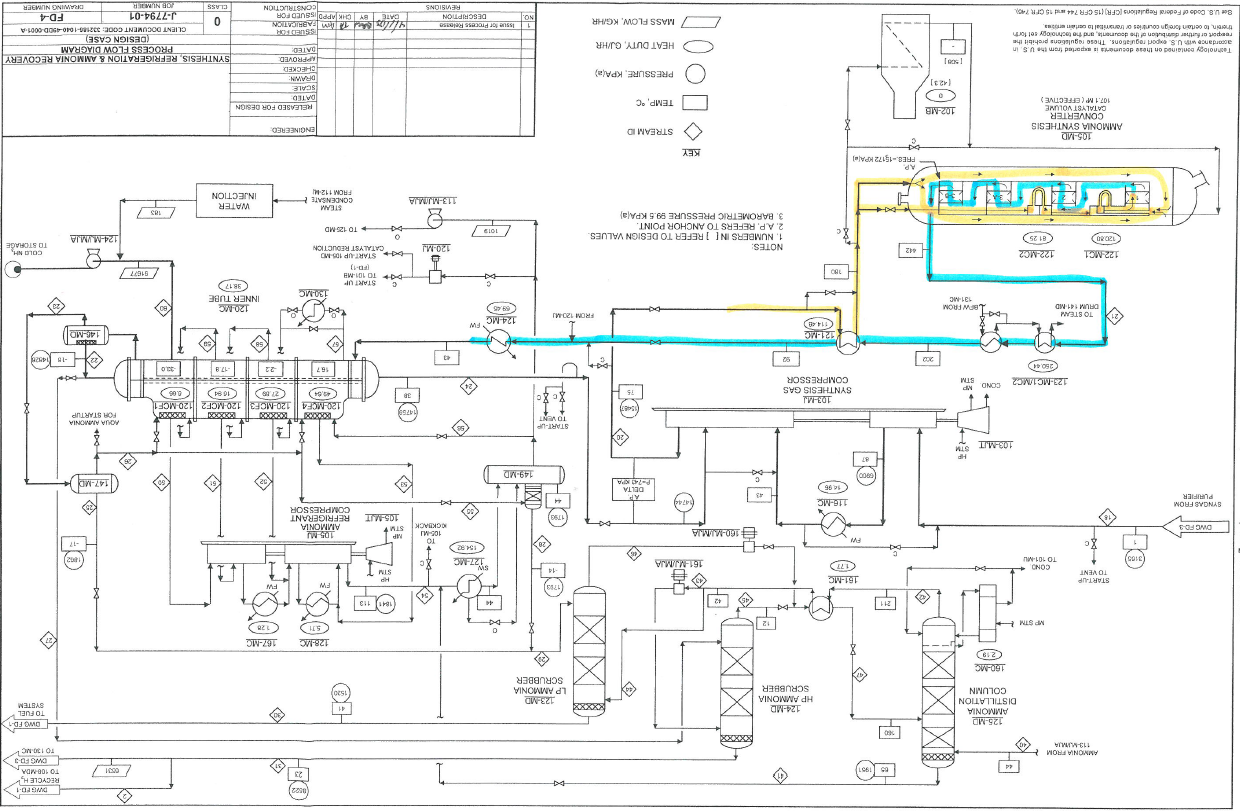
\includegraphics[scale=0.9]{media/pfd1.png}}
	\label{pdf1}
\end{figure}
\newpage

\begin{figure}[htb!]
	\centering
	\rotatebox{-90}{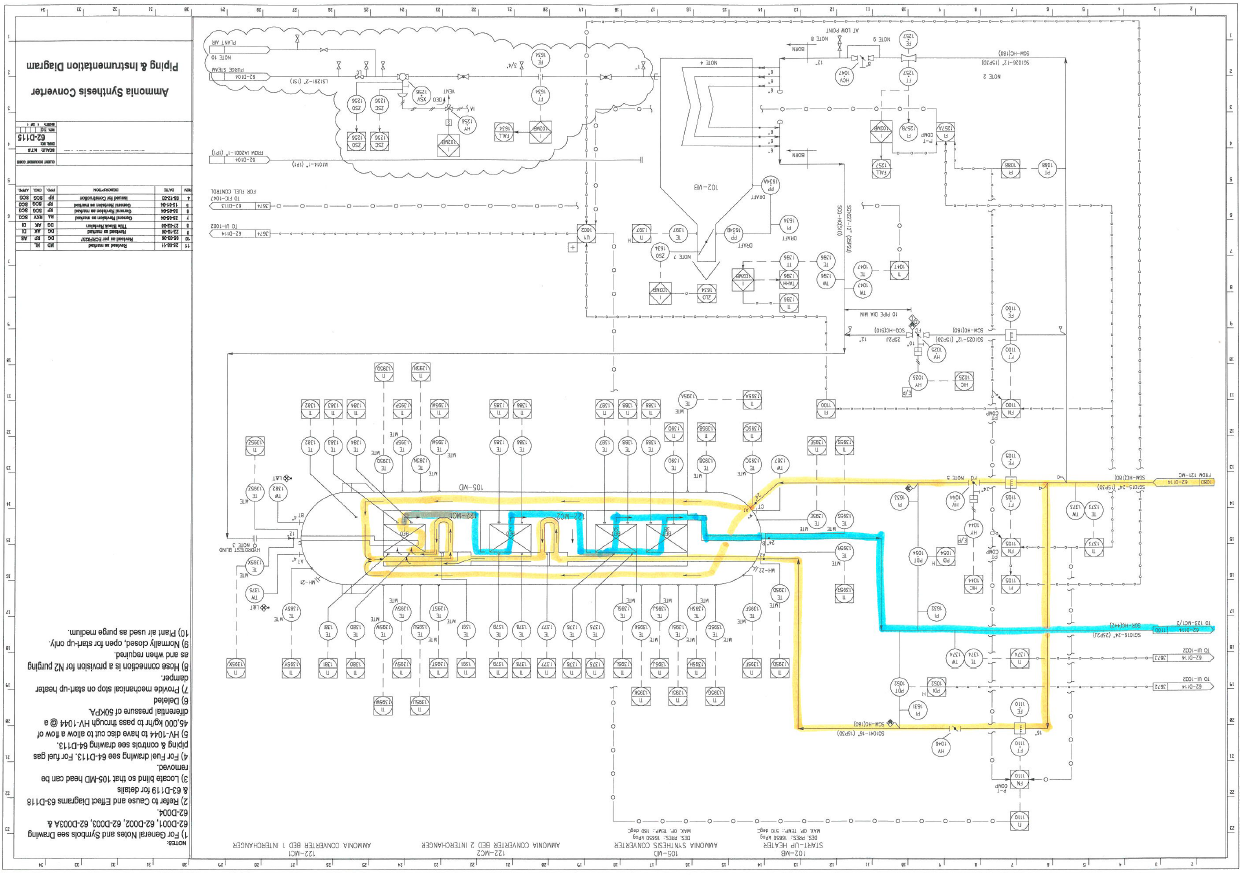
\includegraphics[scale=0.9]{media/pid1.png}}
	\label{pid1}
\end{figure}
\newpage

\begin{figure}[htb!]
	\centering
	\rotatebox{90}{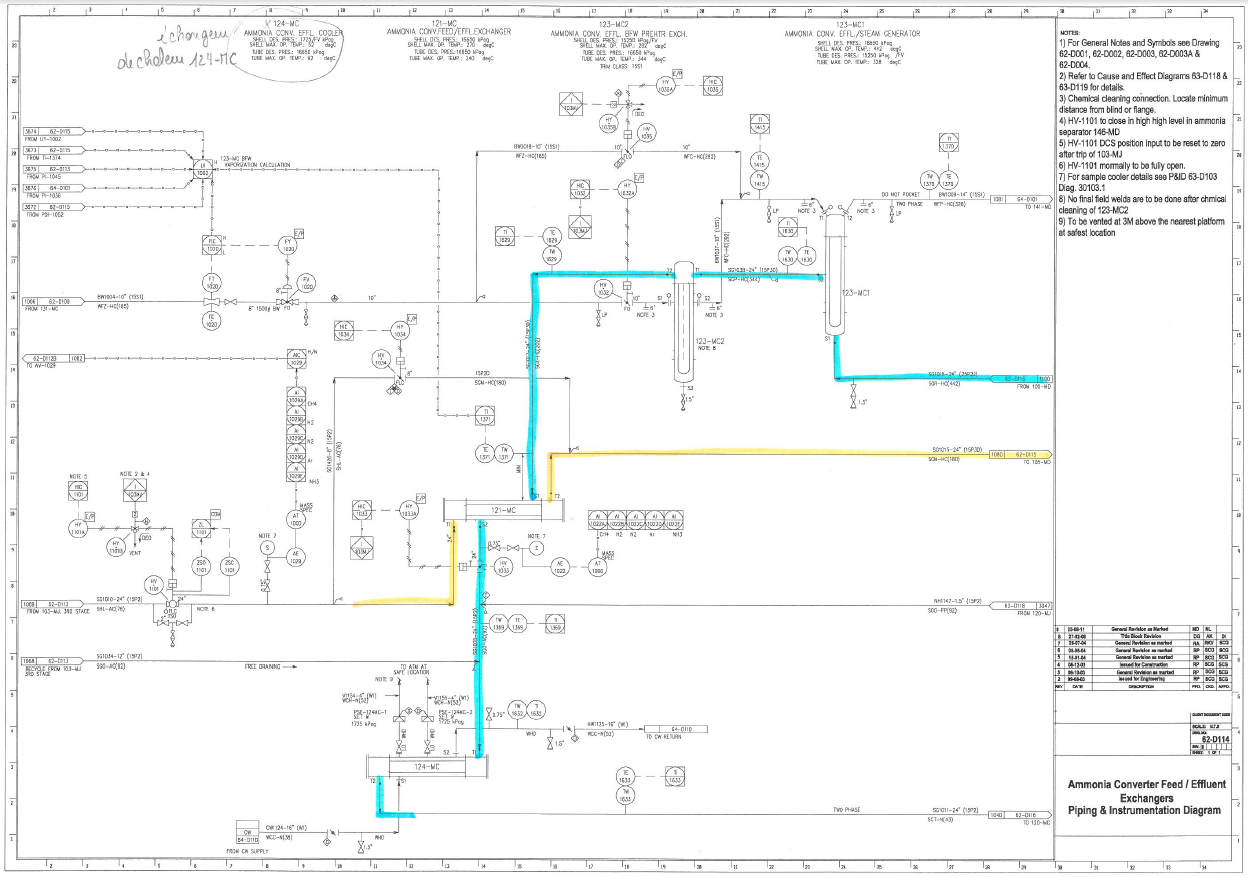
\includegraphics[scale=0.9]{media/pid2.png}}
	\label{pid2}
\end{figure}

\newpage
\section{Analyse HAZOP}
A nouveau, veuillez vous référer à la section \ref{sec:trajectoire}
pour localiser les différents composants cités dans cette section.

	\begin{table}[ht!]
		\centering
		\rotatebox{90}
		{
			\begin{tabular}{|p{0.25\textwidth}|p{0.25\textwidth}|p{0.25\textwidth}|p{0.25\textwidth}|}
				\rowcolor{Gray} Mot-guide		& Causes 	& Conséquences 	&	Mesures de maîtrise 	\\
				\hline
				Trop de corrosion		 
				& Une \textit{hydrogen attack} due à réaction à haute pression 
				de l'hydrogène avec l'acier. Lieu: Du début jusqu'à la chambre 1 du 105MD
				& Les tuyaux sont endommagés (percés ou présence du fuites) ce qui peut
				même mener à une explosion quand l'hydrogène et l'oxygène rentrent en contact. 
				Lieu : Du début jusqu'à la chambre 1 du 105MD.	 
				& Contrôle des matériaux	et augmentation de leur qualité. Prévoir les revêtements adéquats pour éviter tout contact entre acier et hydrogène. 	\\				
				\hline
				Température	trop basse	
				& Liquéfaction/condensation de l'ammoniac juste après le 124MC.	
				& Tuyaux bouchés ce qui peut entrainer une surpression juste après le 124MC.  
				& Installer un dispositif (disque de rupture ou soupape de sécurité) pour contrer
					les problèmes de surpression. \\
				\hline 
				Trop d'usure, corrosion	
				& Dégradation des installations avec le temps et impureté des produits 
				dans les conduits. Lieu: Dans toutes les canalisations mais principalement entre 
				le 105MD et le 123MC1 du à la haute pression.	
				& Entraîne des réactions indésirées qui amènent des impuretés dans l'ammoniac. 
				Lieu : Dans toutes les canalisations mais principalement entre le 105MD et le 123MC1 
				du à la haute pression.	 
				&  Contrôler les installations tous les ans et mettre un filtre physique pour avoir de l'ammoniac pur.	\\
				\hline
				Température trop haute	
				&	Surpression dans le réacteur de synthèse d'ammoniac (105MD).				
				& Peut entrainer des fissures dans la paroie voire même la destruction du réacteur. 
				Il y alors risque d'explosion (105MD).							
				& Présence d'un disque de rupture pour éviter la surpression. \\
				\hline
			\end{tabular}
		}
		\caption{Synthèse de l'analyse HAZOP.}
	\end{table}

\newpage
\biblio{sources-tache4}

\end{document}
